\section{Verwendete Szenen} % (fold)
\label{sec:verwendete_szenen}

	\renewcommand{\arraystretch}{1.3}
	\begin{table}[H]
		\begin{tabularx}{\textwidth}{p{0.35\textwidth}p{0.64\textwidth}}
			\hline
			\textbf{Bild} & \textbf{Daten} \\
			\hline
			\hline \\

			\raisebox{-0.8\totalheight}{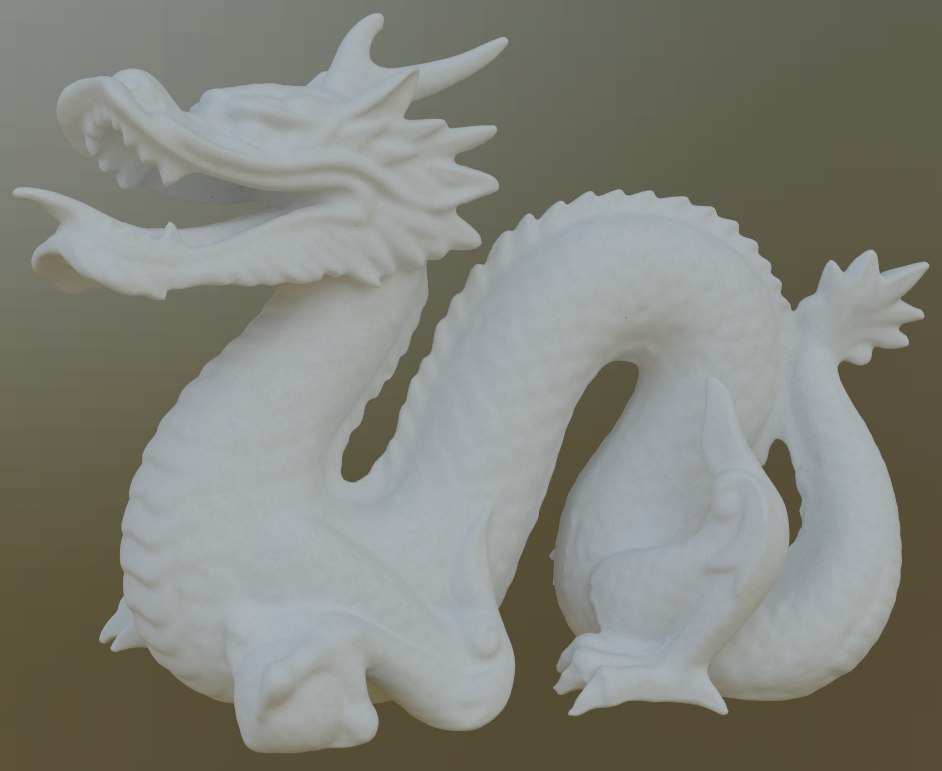
\includegraphics[width=0.3\textwidth]{pic/irr_est-ra-dragon-irr.png}} & \parbox[t]{0.64\textwidth}{\textbf{\enquote{Dragon}-Szene:} \bigskip\\ $871306$ Dreiecke \\ $439704$ Eckpunkte \bigskip\\ Quelle: \cite{scene-dragon,scene-dragon2}} \\
			\\
			\hline \\

			\raisebox{-0.8\totalheight}{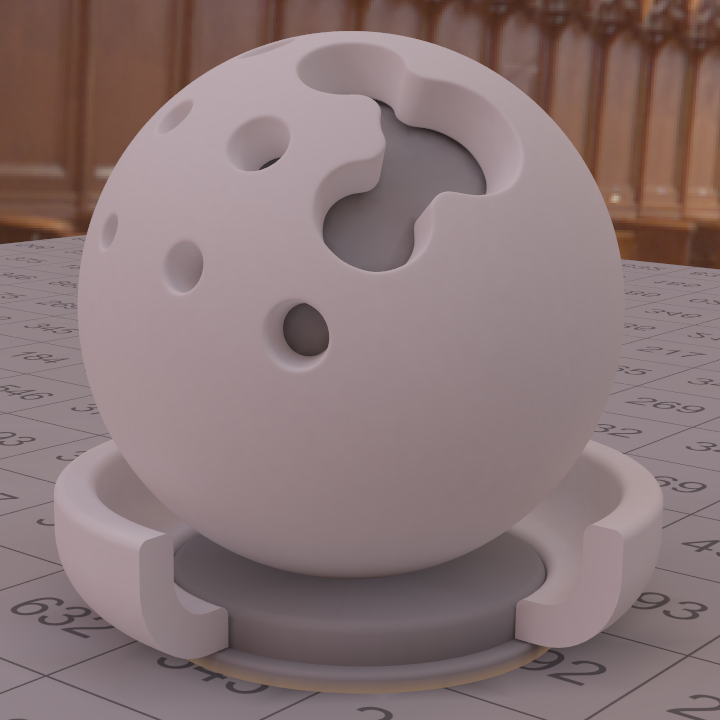
\includegraphics[width=0.3\textwidth]{pic/irr_est-ra-shaderball4-irr.png}} & \parbox[t]{0.64\textwidth}{\textbf{\enquote{Shaderball}-Szene:} \bigskip\\ $119250$ Dreiecke \\ $61258$ Eckpunkte \bigskip\\ Quelle: vom \textit{Fraunhofer ITWM} zur Verfügung gestellt} \\
			\\
			\hline \\

			\raisebox{-0.8\totalheight}{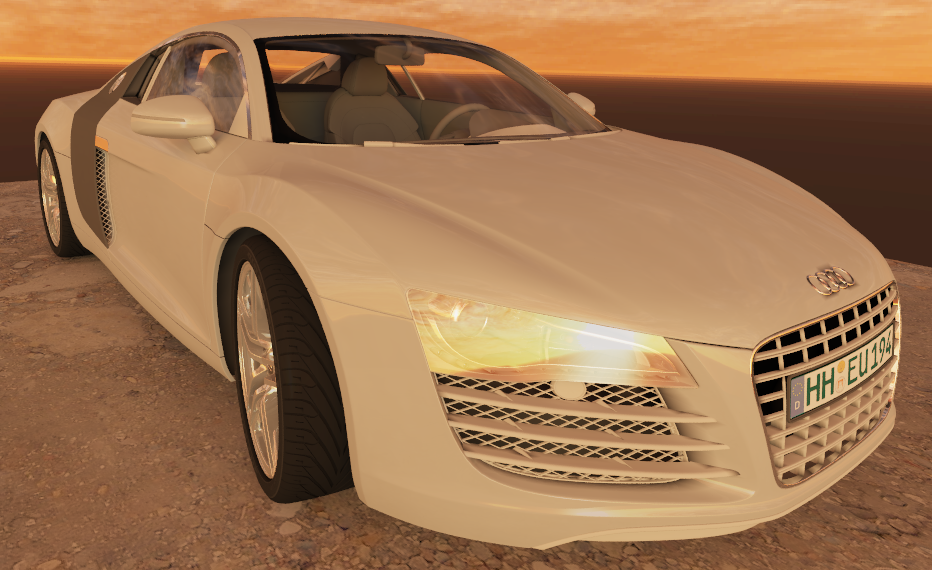
\includegraphics[width=0.3\textwidth]{pic/irr_est-ra-r8-irr.png}} & \parbox[t]{0.64\textwidth}{\textbf{\enquote{Audi R8}-Szene:} \bigskip\\ $1749705$ Dreiecke \\ $1601106$ Eckpunkte \bigskip\\ Quelle: vom \textit{Fraunhofer ITWM} zur Verfügung gestellt} \\
			\\
			\hline \\

			\raisebox{-0.8\totalheight}{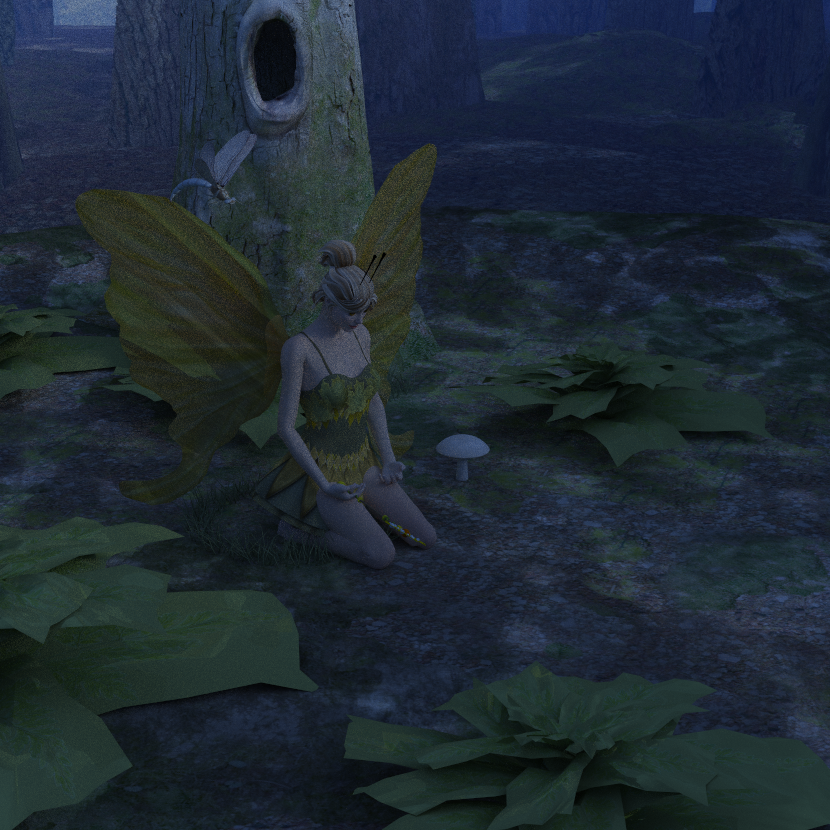
\includegraphics[width=0.3\textwidth]{pic/noise-fairy-low.png}} & \parbox[t]{0.64\textwidth}{\textbf{\enquote{Fairy}-Szene:} \bigskip\\ $174117$ Dreiecke \\ $103523$ Eckpunkte \bigskip\\ Quelle: \cite{scene-fairy}} \\
			\\
			\hline

		\end{tabularx}
	\end{table}

% section verwendete_szenen (end)